\documentclass[a4paper,twoside,11pt]{book}
\usepackage[utf8]{inputenc}
\usepackage[T1]{fontenc}
\usepackage[english]{babel}
\usepackage{amsmath}

\title{Anomaly detection in streaming data using autoencoders}
\author{B.Sc. Bin Li}
\newcommand{\firstprof}{Prof. Dr. Eirini Ntoutsi }
\newcommand{\secondprof}{Prof. Dr. Wolfgang Nejdl}
\newcommand{\betreuer}{Prof. Dr. Eirini Ntoutsi }
\date{\today}
\newcommand{\art}{Master thesis}
\newcommand{\studiengang}{Informatics (M.Sc.)}
\newcommand{\keywords}{Security,Test}

\usepackage{hyphenat}
\hyphenation{Grid--Informations-systeme Sche-du-ler Sche-du-ling Per-for-mance Meta-sche-duler  Pla-gi-ats-prü-fung}

\usepackage{amssymb}							% provides mathmatical math symbols such as dots, arrows, etc.
\usepackage{amsmath}							% provides align environment
\usepackage{listings}
\usepackage{caption}
\usepackage{subcaption}
\usepackage{mathtools}


\lstset{captionpos=b,frame=single}
\usepackage[german]{fancyref}
%% for fancy refereing to listings.
\newcommand*{\fancyreflstlabelprefix}{lst}

\fancyrefaddcaptions{english}{%
  \providecommand*{\freflstname}{listing}%
  \providecommand*{\Freflstname}{Listing}%
}

\fancyrefaddcaptions{german}{%
  \providecommand*{\freflstname}{listing}%
  \providecommand*{\Freflstname}{Listing}%
}

\frefformat{plain}{\fancyreflstlabelprefix}{\freflstname\fancyrefdefaultspacing#1}
\Frefformat{plain}{\fancyreflstlabelprefix}{\Freflstname\fancyrefdefaultspacing#1}

\frefformat{vario}{\fancyreflstlabelprefix}{%
  \freflstname\fancyrefdefaultspacing#1#3%
}
\Frefformat{vario}{\fancyreflstlabelprefix}{%
  \Freflstname\fancyrefdefaultspacing#1#3%
}

%% 1.5 facher Zeilenabstand.
\usepackage[onehalfspacing]{setspace}

\makeatletter
\let\thetitle\@title
\let\theauthor\@author
\let\theday\@date
\makeatother

\usepackage{geometry}
\geometry{a4paper,left=35mm,right=25mm, top=2.5cm, bottom=2.5cm}

% Metadaten
\usepackage[
	colorlinks=true,
	linkcolor=black,						% enable for printing!
	urlcolor=black,						  % enable for printing!
	citecolor=black,						% enable for printing!
	%pdfstartview=Fit,						% fits the page to the window; other options: FitH/FitV (horiz./vert.)...
	%pdfpagelayout=TwoPageLeft,		% the way pages are displayed, options: SinglePage, OneColumn, TwoColumnLeft|Right, TwoPageLeft|Right
	final=true,									% turn on all processing options
	plainpages=false,						% Forces page anchors to be named by the arabic form of the page number, rather than the formatted form.
	pdfpagelabels]							% set PDF page labels
	{hyperref}
\hypersetup{
  pdftitle={\thetitle},
  pdfauthor={\theauthor},
  pdfsubject={\keywords}
}

\usepackage{graphicx}
% sorgt dafür, dass LaTeX in images nach den Bildern sucht und der Ordner "etwas" aufgeräumter ist.
\graphicspath{ {./images/} {./graphics/} }

\usepackage{fancyhdr}
\pagestyle{fancy}
\fancyhf{} % sets both header and footer to nothing
\renewcommand{\headrulewidth}{0pt}
\parindent 0pt

\usepackage{helvet}
\renewcommand{\familydefault}{\sfdefault}
\fontfamily{phv}\selectfont


\setlength{\headheight}{13.6pt}

\begin{document}

\frontmatter
%%%%%%%%%%%%%%%%%%%%%%%%%%%%%%%%%%%%%%%%%%%%%%%%%%%%%%%%%%%%%
%%                                                         %%
%%    Hier sollten von ihrer Seite aus keine Änderungen    %%
%%                  notwendig sein.                        %%
%%                                                         %%
%%%%%%%%%%%%%%%%%%%%%%%%%%%%%%%%%%%%%%%%%%%%%%%%%%%%%%%%%%%%%

\newgeometry{left=3cm,right=4cm, top=3cm, bottom=3.5cm}
\begin{titlepage}

%
% Logos
%

\includegraphics[height=1cm]{logo_dcsec} \hfill

\includegraphics[height=1cm]{logo_luh}

\vspace{-3mm}

\rule{\textwidth}{1pt}

\vspace{5mm}

\large

Gottfried Wilhelm Leibniz Universität Hannover

Institut für Verteilte Systeme

Distributed Computing \& Security Group

\vspace{4.0cm}

\art\\
\studiengang

\vspace{1.0cm}
\huge{\thetitle}

\vfill


\large
\begin{tabular}{p{4cm}l}
Student:    & \theauthor\\
%Verfasser:    & \theauthor\\
First Supervisor: & \firstprof\\
%Erstprüferin: & \firstprof\\
Second Supervisor:  & \secondprof\\
%Zweitprüfer:  & \secondprof\\
%Betreuer:     & \betreuer\\
Date:        & \theday
%Datum:        & \theday
\end{tabular}







\end{titlepage}

\restoregeometry

\cleardoublepage
\newgeometry{left=4.5cm,right=3.5cm, top=4cm, bottom=2cm}
\setcounter{page}{1}
%\section*{Erklärung der Selbständigkeit}
\section*{Declaration of Authorship}
I hereby certify that this thesis has been composed by me and is based on my own work, unless
stated otherwise. No other person's work has been used without due acknowledgement in this
thesis. All references and verbatim extracts have been quoted, and all sources of information have been specifically acknowledged.
\vspace{3cm}


%\rule{6cm}{0.4pt} \hfill Hanover, den \theday\\
\rule{6cm}{0.4pt} \hfill Hanover, \theday\\
\theauthor
\vspace{5cm}

%\section*{Erklärung zur Plagiatsprüfung}
%Mit der Übermittlung meiner Arbeit auch an externe Dienste zur Plagiatsprü-fung durch
%Plagiatssoftware erkläre ich mich einverstanden.

%\vspace{3cm}


%\rule{6cm}{0.4pt} \hfill Hannover, den \theday\\
%\theauthor

\restoregeometry

\fancyfoot[C]{\thepage}

%CONTENTS PAGE
\tableofcontents

\makeatletter
\@openrightfalse
\makeatother

%LIST OF FIGURES PAGE
\listoffigures

%LIST OF TABLE PAGE
\listoftables

%CODE 
\renewcommand*{\lstlistlistingname}{Codeverzeichniss}
\lstlistoflistings


\mainmatter
\renewcommand{\headrulewidth}{0.4pt}
\fancyhead[OR]{\fontfamily{phv}\selectfont \rightmark}
\fancyhead[EL]{\fontfamily{phv}\selectfont \leftmark}

\makeatletter
\@openrighttrue
\makeatother

%%%%%%%%%%%%%%%%%%%% MAINPART%%%%%%%%%%%%%%%%%%%%%%%%%%%%
\chapter*{Abstract}
\addcontentsline{toc}{chapter}{Abstract}
\label{chap:abstract}
The amount and variety of data stream generated from applications of different domain grows steadily and are valuable for big data research. One of the most important core component is the anomaly detection for streaming data, which has attracted attention and investigation in plenty of application areas, for example, the sensor data anomaly detection, predictive maintenance, event detection. Those efforts could potentially avoid large amount of financial costs in the manufacture. However, different from traditional anomaly detection tasks, anomaly detection in streaming data is especially difficult due to that data arrives over time with latent distribution changes, so that a single static model doesn’t fit streaming data all the time. An anomaly could become normal along with data changing in the stream, it is necessary to maintain a dynamic system that deals with this problem. In this paper, we propose a novel LSTMs-Autoencoder anomaly detection architecture specially designed for streaming data. This is a mini-batch based streaming processing approach. We experimented with streaming datasets containing different kinds of anomalies as well as distribution changes, and the results suggest that our model can sufficiently detect anomaly in data stream and update model timely to fit the latest data property.

\chapter{Introduction}
\label{chap:Introduction}

Anomaly detection is a core component of data mining, and widely used in the manufacture, e-commerce, internet applications etc. It could avoid inconvenient and reduce lose in many scenarios like machine health monitoring, credit card fraud detecting and spam email recognition, and could also be used as a preprocessing step to remove anomalies from datasets in many machine learning tasks. There are already plenty of anomaly detection techniques proposed in previous literatures, that solve this problem from variety perspectives, e.g. distance-based methods, clustering analysis, density-based methods etc.\\

There is no lack of anomaly detection approaches that perform good with respect to different kinds of data. Supervised approaches take anomaly detection as a binary classification problem of “normal” instances and “abnormal” instances, and all instance labels should be available in advance. The key difference to other classification problem is the amount of class label is extremely biased to the normal class. In order to avoid doing data augmentation or down sampling, unsupervised approaches are more direct solutions to this problem, which find out the instances that fit least to the majority as the anomalies. Furthermore, in most situations, only partial labels are available, semi-supervised and one-class models are more efficient. They learn the pattern from labeled normal data, test data that not fit the learned pattern perfectly are the anomalies. Different kinds of anomaly detection approaches fit different use cases and data character. However, most of them are batch model, which means, all data should be available in advance. This becomes a shortcoming under today’s big data background. With the rapid development of hardware in the last decade, the situation of data acquisition and analysis has significantly been changed. Specifically, the IoT application. Assume that we collect data from sensors attached to IoT devices, the data comes continuously and everlasting. In the beginning, no static full set of data is available for model initialization in the traditional way. Besides, during data analysis, we should always consider the volume and velocity of data, which means, on one hand, with traditional batch classifiers, the infinity data stream will lead to out of memory, on the other hand, streaming data usually comes in a high speed that leaving the system few processing time, the model should work with only single look at each data point in the stream. In addition, the statistical property of data may also change over time, which is formally called ‘concept drift’. The model should always learn new knowledge from the stream and update its identification of anomaly automatically, while anomalies could be temporally. After a data distribution change, an anomaly possibly becomes normal in the new data environment. Data distribution changes should not be classified as anomaly, and anomaly show up rarely in over the stream, they should also not be oversighted. To this end, an anomaly detection system for streaming data should be able to 1) be initialized with only a small subset, 2) process streaming data and make prediction in real-time, 3) adapt data evolution over time. 4) model should be able to deal with the biased class problem.\\


LSTMs are a kind of recurrent neural network and proposed for temporal dependently data. As a neural network based model, LSTMs can deal with high-dimentional and non-linear data, with arbitary expansion of the model structure. In the last decade, LSTM are used widely in time series prediction, text prediction. And LSTMs-based autoencoder is a good choice for sequence to sequence problem, e.g. language translation, time series data embedding. Deep LSTMs have also shown good performance of capturing hierarchical information from time series like seperation of sentances. Recently, LSTMs-based autoencoders are also used for time series anomaly detection in order to capture the temporal information between data points. For example, Malhotra et al. introduced an autoencoder based anomaly detection approaches in [1],[2], and achieved good performance in multiple time series dataset. However, in those approaches, they still assume that the whole datasets are available beforehand and work on static data. Also, they didn’t consider the aforementioned online learning difficulties. Hence, we enhanced this kind of LSTMs-Autoencoder based static anomaly detection approaches with the online learning ability by implementing incremental model updating strategies with streaming data.\\

Neural networks, including autoencoders, are normally used in batch fashion, namely the whole training set is available, and trained by backpropagation. When come to online setting, only small subset accumulated data from stream are available for model initial training, which may be suboptimal. Assume that the initialization set is enough to train a convergent model, the further streaming data are used for further model updating to adjust latest streaming data changes and the patterns never seen ever. Unlike batch models, instead of aiming at best overall performance, online neural networks are learned to achieve best sequential performance for current streaming data. The difficulty is to detect when model should be updated according to latest data and updating with which part of data. The short-term changes of data distribution should not cause model variation, while permanent concept drifts should trigger model updating as soon as possible.\\

In this paper, we introduce a novel and robust incremental LSTMs-Autoencoder anomaly detection model, which designed specifically for time series data in a streaming fashion using Long Short-Term memory (LSTM) units, with also online learning ability for model updating. For each accumulated mini-batch of streaming data, the autoencoder reconstructs it with previous knowledge learned from normal data. Anomaly data (never used for training) is expected to cause significant larger reconstruction error than normal data. In addition, the model is able to update itself when detected data distribution changes. The LSTMs-Autoencoder is experimented with different data streams, the experiment results shows its ability in detecting anomaly from streaming data and is able to adjust itself with different kinds of concept drifts by model online updating.\\


The rest of this paper is organized as follow. In \autoref{chap:relatedworks}, we collected previous works on anomaly detection and their shortcomings. We also refer some works on incremental neural network. In \autoref{chap:Preliminaries}, define the problem formally. In \autoref{chap:Proposedmodel}, we propose our method for streaming data anomaly detection and discuss the advantage over previous works. In \autoref{chap:Experimentalsetup}, we describe the datasets used for experiments and the experimental set-up. In \autoref{chap:results}, we present our experimental results. And in \autoref{chap:conclusion}, we summarize the work and discuss of success and deficiency.

\chapter{Related works}
\label{chap:related works}

In this section, we present a survey on previous works in anomaly detection with classical machine learning models and with autoencoders, as well as studies of neural network updating along with streaming data.

\section{Batch model}
\label{sec:batch}

\subsection{Classical machine learning based approaches}
\label{sec:classical}

As an important component of data mining and machine learning, anomaly detection has been investigated using plenty efficient models. When talking about anomaly detection, the most intuitive solution may be detection of outliers from a dense cluster, or to find thoes data points that have obvious different property as their neighbors and so on. Within thoes large batch of classical methods, the Local Outlier Factor (LOF) and One-class Support Vector Machine (OCSVM) are two commonly used models in real-world use cases.

\subsubsection{Local outlier factor}
\label{lof}
In anomaly detection, the LOF is a common density-based approach. LOF shares some concepts with DBSCAN such as ‘core distance’ and ‘reachability distance’, in order to estimate local density. Here, points with substantially lower local density than their neighbors are considered as anomalies. LOF shows competitive performance in many anomaly detection tasks, especially when dealing with data with unevenly density distribution. However, when getting a numerical factor from LOF model, it is actually hard to define a threshold automatically for the judgement of anomaly.\\\\

\subsection{One-class SVM}
\label{ocsvm}
Another widely used model is the domain based One-class Support Vector Machine. As an unsupervised one-class classifier, OCSVM takes only normal data as input, and generates a decision surface to separate them from the anomaly states. By analyzing anomalies, the datasets are always bias to the normal part, and anomaly appear only rarely. So, this kind of one-class classifiers avoid making balance between the two classes. Besides, they also take advantage of classical support vector machine, with the help of kernel method, they can also deal with linearly not separable data. However, in the mean time, the choosing a proper kernel becomes a hard point of OCSVM. A suboptimal kernel function can seriously impact the performance.\\
Although classical machine learning approaches can handle most of the normal anomaly detection, there a still a lack of pervasive models that fit different kinds of data characters. Moreover, only few of those approaches could be directly or after some modification used for time series and streaming data, while they ignore the temporal dependency between samples.




\section{Autoencoder-based anomaly detection approaches}
\label{sec:Autoencoder-based anomaly detection approaches}

LSTMs-Autoencoders are originally widely used for text generation. Text data are usually embedded into vector as input of autoencoder. And the tasks are either generate temporal relevant text on the decoder side or learn text representation in the hidden layer \cite{phraserepresentation}. As text data are relevant in the sense of words within a sentence or between sentences, it is similar to the streaming data temporal dependency problem.\\

Sutskever et al. \cite{seq2seq} use a deep LSTMs-based sequence to sequence model for language translation. In their work, the deep LSTMs encoder take single sentence as input, and learn a hidden vector of a fixed dimensionality, and then a different LSTMs decoder decodes it to the target sentence.  As a translation task, they found that this encoder-decoder architecture can capture long sentences and sensible phrases, especially they achieved better performance with deep LSTMs in compare with shallow LSTMs. In addition, a valuable found is, reversing the order of words in the input sentence makes the optimization problem much easier and achieved better performance. The LSTMs based model outperforms non-LSTMs model on the long input sentence cases (more than 35 words) since its long-term memory ability.\\

Li et al. \cite{hierarchicalseq2seq} did similar research on long paragraph text and even entire document generation using LSTMs-autoencoders. Their main contribute is the hierarchical sentences representation. The model learns words level, sentence level and paragraph level information with each respectively a LSTMs layer, so that the model captures very long-term temporal information. Moreover, they introduced an attention based hierarchical sequence to sequence model that connect the most relative part between encoder and decoder like the works around a final punctuation. They experiment with documents over 100 words, the results show that hierarchical and attention-based hierarchical LSTMs learns even better long-term temporal information than standard LSTMs-encoder-decoder models.\\

As autoencoders achieves great successes in text data and speech processing, they are also used on time series anomaly detection in terms of temporal dependently data. These models train autoencoders with only normal data, and anomaly data as unknown patterns. Then the autoencoder can only reconstruct normal patterns, large reconstruction error indicates anomaly. An early work \cite{eps} uses the vanilla autoencoder to detect abnormal status of the electric power system. In order to capture temporal information, they applied sliding window on the raw data as input. As anomaly scoring method, they evaluated each sliding window with respect to their reconstruction error. As some measures in the autoencoder output vectors are more sensible to anomalies than others, they use the average absolute deviation of reconstruction error as anomaly score. And the anomaly threshold is chosen by large amount of experiments over normal data.\\

An important reason of using autoencoder for anomaly detection is its ability of dealing with high-dimensional. Sakurada et al. \cite{ dimensionalityreduction} experimented with time series data that consist of 10-100 variables with no linear correlation. Comparing with reconstruction using PCA or Kernel PCA techniques, using the autoencoder reconstruction error is more easily to recognize anomalies.\\

In further researches, Malhotra et al. \cite{lstmad}\cite{encdecad} develop the application of LSTMs-autoencoder in sequence learning into anomaly detection problem. They proposed stacked LSTM networks model to learn high level temporal patterns. They show that LSTMs outperforms normal RNNs based anomaly detection model and avoid facing to the gradient vanishing problem. They also detect anomaly based on the reconstruction error. The scoring function is based on the parameters of a estimated normal distribution of a validation set. Their experiments show that the model performs good in variety kinds of datasets. A variation of this model \cite{timenet} has been proved that achieves better performance in the anomaly detection tasks, while they tell that using a constant as input of decoder instead of read time series value improves the performance of model.


\section{Online incremental learning with autoencoders}
\label{sec:Online incremental learning with autoencoders}

Zhou et al. \cite{online} proposed an online incremental updating method for denoising autoencoders by modifying the hidden layer neurons in order to deal with the non-stationary streaming data properties. The kern ideal are two steps, adding hidden layer neurons to capture new knowledge, and merging hidden layer neurons if information is redundant. Their experimental result shows comparable or better reconstruction result than non-incremental approaches with only few data used during initialization. And they show that their incremental feature learning methods performs more adaptively and robustly to highly non-stationary input distribution.\\

Dong et al. \cite{threaded} proposed a 2-step anomaly detection mechanism with incremental autoencoders. The implemented the system with ensembled autoencoders in multithreads to leverage parallel computing when large volumes of data arrive. Besides their 2-step mechanism check anomaly in the first step and verify anomaly data with previous and subsequent data (to differ between anomalous state and concept drift) to reduce false-positive rate in anomaly detection. In the experimental results, they show that their model outperforms commonly used tree-based anomaly detection model especially when concept drift presents and speed up the online processing speed with mini-batch learning and online learning in multithreads.\\

In this work, we implement a LSTMs-autoencoder based incremental streaming data anomaly detection model. The LSTMs-autoencoder is close to the model by Malhotra et al. \cite{encdecad}, and we design an online model updating strategy as well as the dataset used for model updating.








\chapter{Preliminaries}
\label{chap:Preliminaries}

In this section, the streaming data and the model basic will be introduced. At first, we formally define a data stream used in the experiments. Furthermore, we figure out the definition of anomalies in streaming data, and metrics to evaluate anomaly detection. And finally we refer the main concept of autoencoders and LSTMs, which are the basic architecting and component of our model. \Fref{tab:noration} is a summarization of notations used in this section.

\begin{table}[h]
\begin{center}
\begin{tabular}{|l|l|}
\hline
Notation & Description \\ \hline
DS & Data stream \\
$x_{T}$ & Instance arrived at time T \\
$t_T$ & Timestamp of time \\
MB & Batch size	\\	
$c \in R^hs$ & LSTM unit cell state with hs dimensions \\
a & Cell output  \\ 
$\chi = R^d $ & Feature space with d dimensions  \\
X & A random variable take values from $\chi$	\\
$\Phi$ & Shaping function of autoencoders	\\	
$\Psi$ & Activation function of autoencoders	 \\
H & Hidden layer representation of autoencoders  \\
$d_T$ & Decoder input at time \\  \hline


\label{tab:notation}
\end{tabular}
\end{center}
\end{table}


\section{Definition of stream}
\label{sec:Definition of stream}

Assume that a set of devices or data warehouses generate data continuously (here we only take about numerical data). A data stream DS is defined as 
\begin{equation} \label{eq:DS}
DS = \{(x_1,t_1),(x_2,t_2), ... , (x_T,t_T), ...\}
\end{equation}
where \textbf{$x_T$} is the instance arrived at timestamp \textbf{$t_T$} and represented by a multi-dimensional vector.\\

In order to feed the streaming data to LSTMs, the stream is accumulated to windows and batches as \Fref{fig:stream}. Every T instances are accumulated to a window as a single LSTM input. And MB is the predefine batch size, each batch contains MB windows.\\

\begin{figure}[h]
\centering
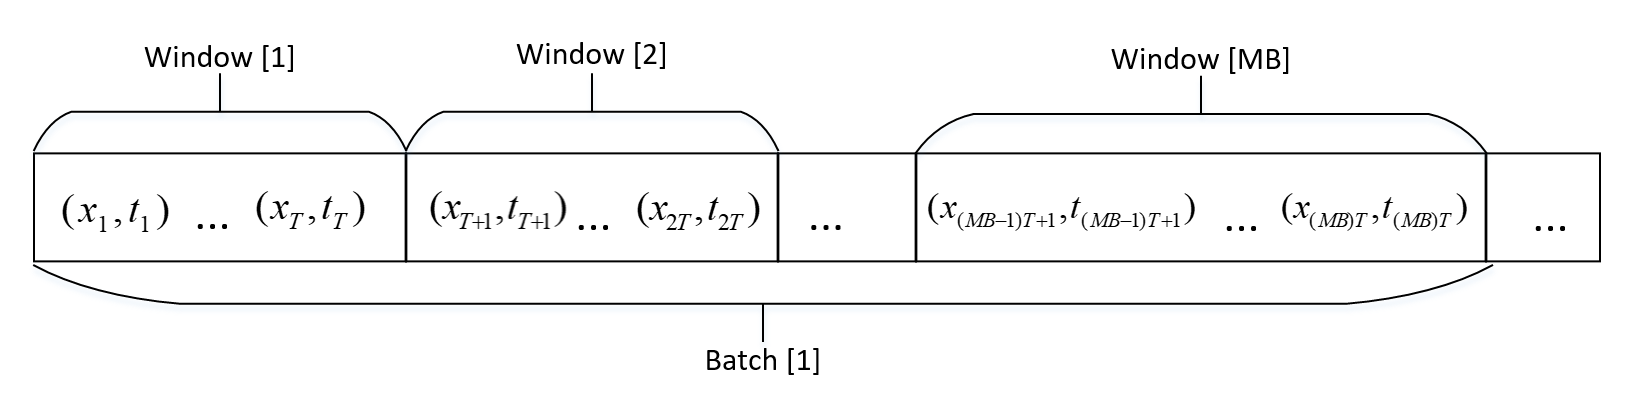
\includegraphics[width=12cm, height=3cm]{stream}
\caption[Data stream]{Data stream}
\label{fig:stream}
\end{figure}




\section{Definition of anomalies}
\label{sec:Definition of anomalies}

\textbf{Pointwise}: A data point (instance) is anomalous(e.g. \Fref{fig:point}) if this point is distant from other observations according to some specific measurement metrics. This is used in fine-grained anomaly detection tasks, that need to find out every single anomalous instance, e.g. credit card fraud detection, spam email detection.\\

\textbf{Window-based}: Sometimes, a data point is apparently normal, but this point, or potentially together with its neighbors violates the overall periodicity or other character of the time series, we also treat them as anomaly, which is called window-based anomaly or contextual anomaly, e.g. \Fref{fig:window}.\\
\begin{figure}[h]
\centering
	\begin {subfigure}[t]{8cm}
	\centering
	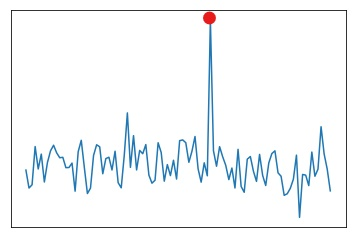
\includegraphics[height=6cm]{anomaly_point}
	\caption{Pointwise anomaly}
	\label{fig:point}
	\end{subfigure}
	~
	\begin {subfigure}[t]{8cm}
	\centering
	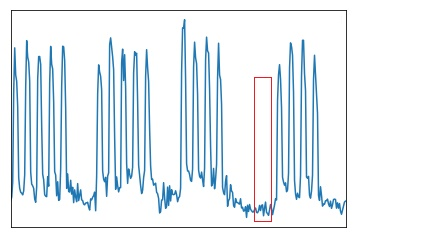
\includegraphics[ height=6cm]{anomaly_window}
	\caption{Window-based anomaly}
	\label{fig:window}
	\end{subfigure}
	\caption[Anomaly types]{Anomaly types}
\label{fig:anomalytypes}

\end{figure}




In the anomlay detection experiments, abnormal data is the object of study, therefore we take the anomaly as positive class and normal data as negative class. \\

\begin{table}[h]
\begin{center}
\begin{tabular}{l|l|c|c|}
\multicolumn{2}{c}{}&\multicolumn{2}{c}{Actual value}\\
\cline{3-4}
\multicolumn{2}{c|}{}&Normal&Abnormal\\
\cline{2-4}
\multirow{2}{*}{Prediction}& Normal & $TN$ & $FN$\\
\cline{2-4}
& Abnormal & $FP$ & $TP$\\
\cline{2-4}
\end{tabular}
\end{center}
\label{tab:conf}
\caption{Confusion matrix}
\end{table}

The target is to achieve higher true positive rate (equation \ref{eq:tpr}, true alarms) while remain lower false positive rate (equation \ref{eq:fpr}, wrong alarms). The evaluation metric is Area Under the Curve (AUC), where the curve is receiver operating characteristic curve, and is created by plotting the true positive rate against the false positive rate at various threshold settings. The range of AUC is between 0 and 1, 1 is the optimal result.\\
\begin{equation} \label{eq:tpr}
TPR =\dfrac{TP}{TP+FN}
\end{equation}

\begin{equation} \label{eq:fpr}
FPR = \dfrac{FP}{FP+TN}
\end{equation}



\section{LSTMs}
\label{sec:LSTMs}

Recurrent neural networks(RNNs) are widely used for speech, video recognition and prediction due to its recurrent property that captures the temporal dependency between data points in compare with other feed forward networks. However, the volume of RNN’s memory is limited, and vanishing gradient is also a difficulty by training RNNs. Therefore, the long short-term memory networks (LSTMs) are a kind of reinforced RNN that are able to remember valuable information in arbitrary time interval. A LSTM network is a recurrent neural network with neurons being LSTM units. \Fref{fig:lstmunit} shows a classical structure of a LSTM unit. LSTMs are able to capture long-term memory while there are a forget gate and a update gate in the LSTM unit, that select necessary previous information and new coming information according to the input data at each time step. The information is transferred to the next step along with the cell state. Besides, each LSTM units also output its value respectively.\\

\begin{figure}[ht]
\centering
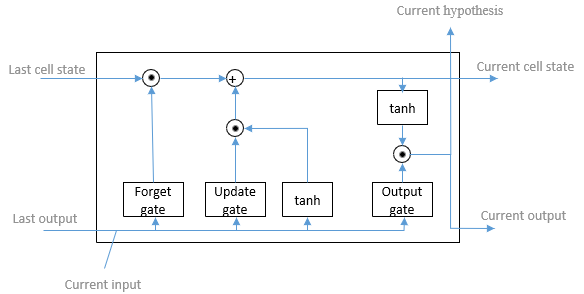
\includegraphics[width=12cm, height=8cm]{lstmunit}
\caption[LSTM unit]{The LSTM unit}
\label{fig:lstmunit}
\end{figure}


A LSTM unit can be unfolded over time, as shown in \Fref{fig:unfolded}. The LSTM unit takes a data window as input (one instance at each time step). Therefore, the LSTM unit extracts useful and drop useless temporal information from the window.\\


Deep LSTM RNNs are built by stacking multiple LSTM layers. Note that LSTM RNNs are already deep architectures in the sense that they can be considered as a feed-forward neural network unrolled in time where each layer shares the same model parameters. It has been argued that deep layers in RNNs allow the network to learn at different time scales over the input\cite{deep}. \Fref{fig:deeplstm} is a example of stacked deep LSTM neural network, there are 3 LSTM layers, each can be unfolded into 5 time steps, so the LSTMs take a window in length 5 as input and the output is in same size.\\

\begin{figure}[h]
\centering
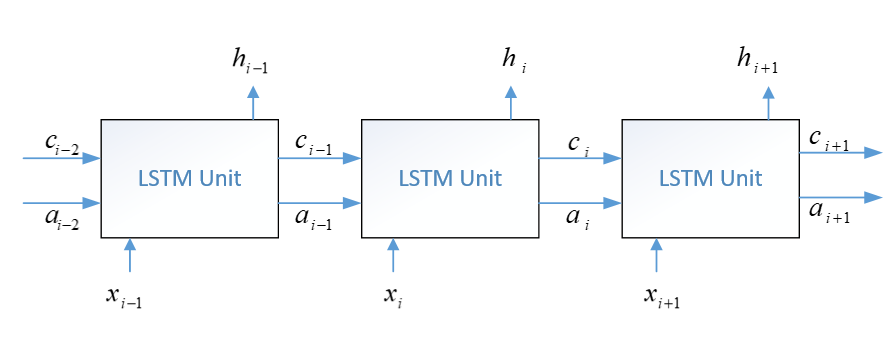
\includegraphics[width=12cm, height=5cm]{unfold}
\caption[Unfolded LSTM unit]{Unfolded LSTM unit}
\label{fig:unfolded}
\end{figure}

\begin{figure}[h]
\centering
	\begin {subfigure}[t]{0.45\textwidth}
	\centering
	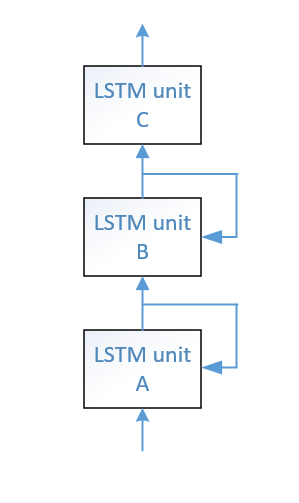
\includegraphics[height=6cm]{deepfolderedlstm}
	\caption{Deep folded LSTMs}
	\label{fig:deeplstm1}
	\end{subfigure}
	~
	\begin {subfigure}[t]{0.45\textwidth}
	\centering
	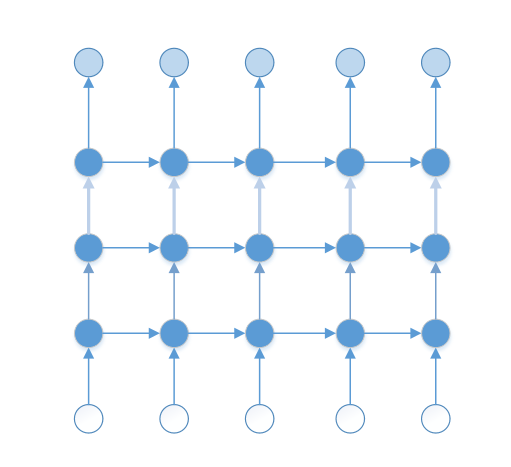
\includegraphics[ height=6cm]{deeplstm}
	\caption{Deep unfolded LSTMs. Each horizontal dark dot chain is an unfoldered LSTM unit over time, hollow dots and grey dots are windows of inputs and outputs.}
	\label{fig:deeplstm2}
	\end{subfigure}
	\caption[Deep LSTMs]{Deep LSTMs}
\label{fig:deeplstm}

\end{figure}

\section{Autoencoders}
\label{sec:Autoencoders}

An autoencoder (\Fref{fig:autoencoder}) is an artificial neural network with symmetrical structure. Normally an autoencoder has at least one hidden layer that consists of less neurons than input and output layers. And the basic aim of autoencoders is to reconstruct its own input and learn a lower dimensional representation (encoding) of input data in the hidden layer. Moreover, the autoencoders are also used for anomaly detection by measuring the reconstruction error between inputs and predictions.
Normally the component between input layer and hidden layer is called encoder, and the symmetrical component between hidden layer and output layer is called decoder. For input $\chi$, the objective function is to find weight vectors for encoder and decoder to minimize the reconstruction error (Equation \ref{eq:autoencoder}).\\

\begin{figure}[h]
\centering
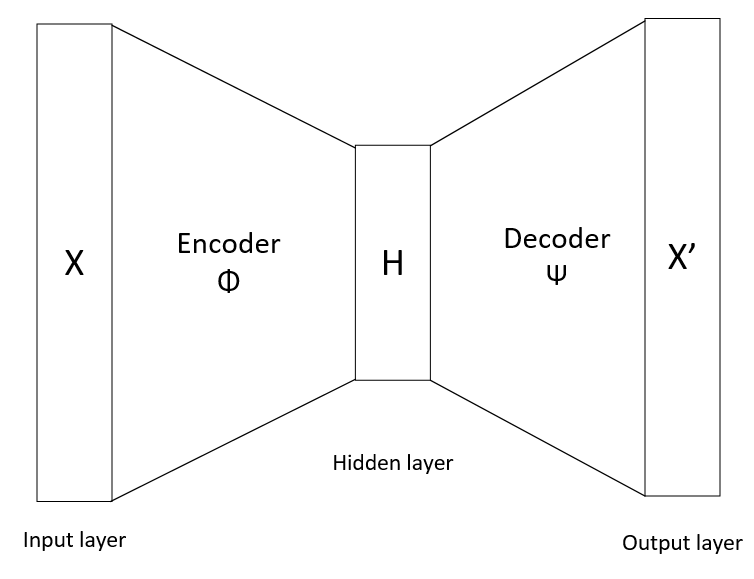
\includegraphics[width=7cm, height=5cm]{autoencoder}
\caption[Autoencoder]{Autoencoder}
\label{fig:autoencoder}
\end{figure}

\begin{equation} \label{eq:autoencoder}
\begin{aligned}
\Phi : &\chi \rightarrow H \\
\Psi : &H \rightarrow \chi \\
\Phi, \Psi = &argmin \left \| X-(\Psi \circ \Phi)X \right \|^2
\end{aligned}
\end{equation}

LSTMs-autoencoder has the same encoder-decoder architecture, while the neurons are LSTM units and connected in the way described in section \ref{sec:LSTMs}. \Fref{fig:encdecad} is a basic LSTMs-based autoencoder architecture with single LSTM layer on both encoder and decoder side. Our incremental LSTMs-autoencoder is based on this structure. The model takes window with length T as input (one instance at each step). The cell state carries sequence information and is passed through LSTM unit over time. When the encoder reaches the last encoder state, namely ET in \Fref{fig:encdecad2}, its cell state is actually the fix length embedding of the input window, and will be copied to the decoder as initial cell state of decoder, so that the input information is also transferred to the decoder. And the decoder predict the window in reversed order in order to make the optimization problem easier. To be notice is, different from aforementioned deep LSTMs in section \ref{sec:LSTMs}, the encoder outputs at each time step are not directly used as inputs of decoder, while between the encoder and decoder is actually not the same logical connection as stacked LSTMs. Here, the outputs of encoder are ignored, and there are different works contributes to the research of decoder inputs. Cho et al. \cite{phraserepresentation} feeds the input sequence to the decoder for a learning phrase representation task, Malhotra et al. \cite{encdecad} feed to decoder LSTM unit at each time step the value of previous time step as input, and in a extended work \cite{timenet} they feed the decoder always a constant vector for an anomaly detection task, because the finial cell state already carries all relevant information to represent the input window. In our model, we feed the decoder a constant vector.\\

\begin{figure}[t!]
\centering
	\begin {subfigure}[t]{0.45\textwidth}
	\centering
	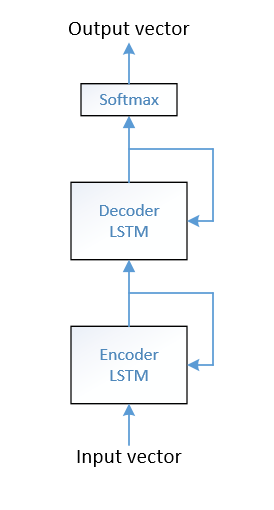
\includegraphics[height=6cm]{folded_encdecad}
	\caption{Folded LSTMs-Autoencoder}
	\label{fig:encdecad1}
	\end{subfigure}
	~
	\begin {subfigure}[t]{0.45\textwidth}
	\centering
	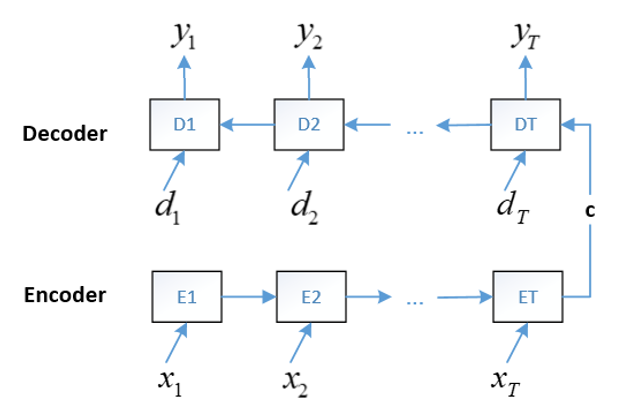
\includegraphics[ height=6cm]{encdecad2}
	\caption{Unfolded LSTMs-Autoencoder}
	\label{fig:encdecad2}
	\end{subfigure}
	\caption[LSTMs-Autoencoder]{LSTMs-Autoencoder}
\label{fig:encdecad}

\end{figure}







\chapter{Proposed model}
\label{Proposed model}

\section{Framework overview}
\label{sec:framework}

The proposed model is a full flow from data stream generation, anomaly detection with autoencoder-based model and online model incremental updating. Apache Kafka is used as the stream generator as shown in \Fref{fig:kafka}. The first received batches of streaming data are used for decision of model hyperparameters and the model initialization. Hyperparameters includes the hidden layer size, batch size, input window length as well as the number of epochs. Once the hyperparameters are learned, an autoencoder will be constructed and initialized with random weights. A subset of the streaming data is used for initial model training (only normal data used for training). Furthermore, the model is used for online anomaly detection, and will be retrained when the retraining condition is triggered. As aforementioned, topic is the data category mechanisms in Kafka. The streaming data are published to a topic, and the prediction results are send back to another Kafka topic for visualization.

The Consumer 2 in \Fref{fig:kafka} is actually the core component of the LSTMs-autoencoder model. Once the initialized model is available, the online phase is then start. As shown in Algorithm \ref{alg:pipeline}, if a batch of streaming data is available, the model will start do prediction, evaluation, and check whether current batch is useful to store for later retraining. 


\begin{figure}[h]
\centering
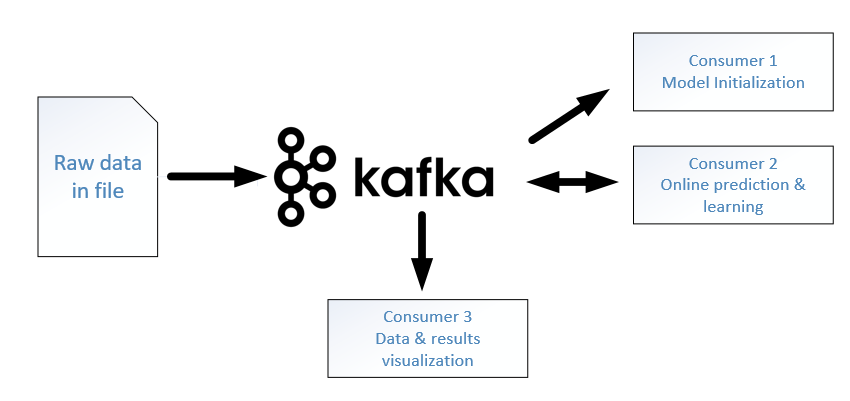
\includegraphics[width=10cm, height=5cm]{kafka}
\caption[Data stream pipeline]{Data stream pipeline}
\label{fig:kafka}
\end{figure}

\begin{algorithm}[t]
\SetKwInOut{Input}{input}
\Input{performanceThreshold, retrainDataSize}

\BlankLine 
needRetraining = False\;
retrainBuffer = [ ]\;
 \While{Batch data available}{
  batch, label = getBatchData()\;
  \eIf{len(retrainBuffer) == retrainDataSize}{retrain(retrainBuffer)\;}
	{
   	pred = predict(batch)\;
	result = evaluation(pred,label)\;
	\eIf{result >= performanceThreshold}{continue\;}{\eIf{label == "normal"}{retrainBuffer.append([B, label])\;}{continue\;}}
	}
 }
 \caption{Pipeline}
\label{alg:pipeline}
\end{algorithm}



\section{LSTMs-Autoencoder initialization}
\label{sec:initialization}

\subsection{Encoder-decoder architecture}
\label{sec:Encoder-decoder architecture}

The LSTMs-Autoencoder is consist of two LSTM units, one as encoder and the other one as decoder. The encoder inputs are fix length vectors with shape <MB, T, D>, where MB is the number of data windows contained in a mini-batch, T is the numbers of data points within each data window, and D represents the number of data dimensionality. Here, MB and T are learned as hyperparameter in the initialization phase. And on the decoder side, it will output exactly the same format data vector for each mini-batch. The LSTM unit copies its cell state for itself as one of the cell input at next timestamp. At the last timestamp of encoder, the cell state of LSTM unit is the hidden representation of the input data vector and copied to the decoder unit as initial cell state, so the hidden information can be passed to the decoder. The size of hidden layer representation vector, namely the size of cell state is another hyperparameter need to be learn in the initialization phase. The larger the hidden vector, the more information can be captured during the process, so it is a feature highly depends on the data. Similar to previous study \cite{seq2seq}, we also train the encoder and decoder with time series in reverse order. For example, if the input data fragment are data points from timestamp t1 to t2, then the decoder will predict data point at t2 at first, and then back to t1 step by step, while this trick makes the gradient escarpment between last state of encoder and first state of decoder smaller and easier to learn. \\

In order to let the whole process happen online, the model initialization also utilizes streaming data. Once a small subset of streaming data is available, hyperparameters are learned, and then another dataset that consists only of normal data is collected from stream used for training. Assume that once an anomaly detection task is determined, the anomalous state is explicit defined and a subset of anomalous data is available for model initialization. We split the normal data into four subsets, $N_1$ for hyperparameters tuning, $N_2$ for model training, $N_3$ for early stopping, and scoring parameters learning, $N_4$ for testing. And abnormal data are split into two subsets, $A_1$ for decision of anomaly score threshold, $A_2$ for testing.

\subsection{Anomaly detection mechanism}
\label{anomalydetection}
The autoencoder reconstructs the input with its knowledge of normal data, so if the input data contains anomalies, the reconstruction error will be obviously large due to the lack of anomalous knowledge. For input $X^{(i)}$, the reconstruction error is 

\begin{equation} \label{eq:error}
e^{(i)}=\left| X^{(i)} - X^{'(i)} \right|
\end{equation}

similar to \cite{encdecad}, the reconstruction error of data points $N_3$ is used to estimate the parameters $\mu$ and $\Sigma$of a normal distribution $\mathcal{N}(\mu,\,\Sigma)$ using maximum likelihood estimation. The anomaly score for a point $x_t^{(i)}$ is defined as 

\begin{equation} \label{eq:score}
a^{(i)}={(e^{(i)}-\mu)}^{T}{\Sigma}^{-1}{(e^{(i)}-\mu)}
\end{equation}

During the initialization phase, a anomaly score threshold $\tau$ is also learned using $N_3$ and $A_1$ as

\begin{equation} \label{eq:threshold}
\tau = argmax Auc(a(N_3),a(A_1))
\end{equation}




\section{Online learning}
\label{sec:Onlinelearning}
However, if we consider using the model for streaming data, the autoencoder might get outdated because of the relative small and simple initialization dataset and concept drift happed along with time. So the update of model is necessary. The main contribution of this paper is the incremental learning setting of the autoencoder model.

\subsection{Retraining trigger}
\label{trigger}

\subsection{Retraining dataset}
\label{data}



\chapter{Related works}
\label{chap:related works}


\section{Classical machine learning based approaches}
\label{sec:Classical machine learning based approaches}




\section{Autoencoder-based anomaly detection approaches}
\label{sec:Autoencoder-based anomaly detection approaches}







\chapter{Experimental results}
\label{chap:results}


\section{Anomaly detection performance}
\label{sec:performance}

With parameters learned from \Fref{sec:parametertuning}, autoencoders are trained for each dataset with the beginning of streaming data. The anomaly detection performance is indicated by AUC. For each dataset, we compare the AUC of online phase that without and with continuously model and parameter updating (\Fref{tab:performance}). For the PowerDemand dataset, retrain trigger depends on the batch performance. And for the rest datasets, retraining only triggered when retrain buffers are full. The retraining brings overall performance improvement on all datasets comparing to stationary models. Especially in the SMTP+HTTP dataset, the stationary without learning concept drifted knowledge performs clearly worth than the model with updating.

\begin{table}[h] 
\caption{Performance} 
\centering      
\begin{tabular}{c | c | c | c}  
\hline  
Dataset & AUC(without retraining) & AUC(with retraining) & \#retrain \\ 
\hline 
PowerDemand & 0.91 & 0.97 & 2  \\  
\hline 
SMTP & 0.94 &  0.98 &  2 \\ 
\hline 
HTTP & 0.76 &  0.86 &  2 \\ 
\hline
SMTP+HTTP & 0.64 & 0.85 & 3 \\
\hline 
ForestCover &0.74&0.82 & 8\\   
\hline    
\end{tabular}
\label{tab:performance}  
\end{table} 
In order to compare the performance with and without retraining, after each model updating, we calculate the AUC value for each specified time period. As Shown in \Fref{fig:auc_retrain}, the x-axis represents the periods, for example, before first retraining(shown as P1 in each subplot), between first and second retraining (P2), and so on. For each dataset, we compare the AUC value of stationary model (trained with only initialization set) and adaptive model (online updated). For most cases, the adaptive models outperform stationary models, which shows the models profits from the knowledge updating over streaming data. To be notice that the SMTP+HTTP set contains sudden concept drift around P3, which leads to a sharp decline of the stationary model. In the meantime, the adaptive model is only slightly influenced by the mixed knowledge at P3 but keeps outstanding performance when the stream switches to HTTP side.\\
\begin{figure}[h]
\centering
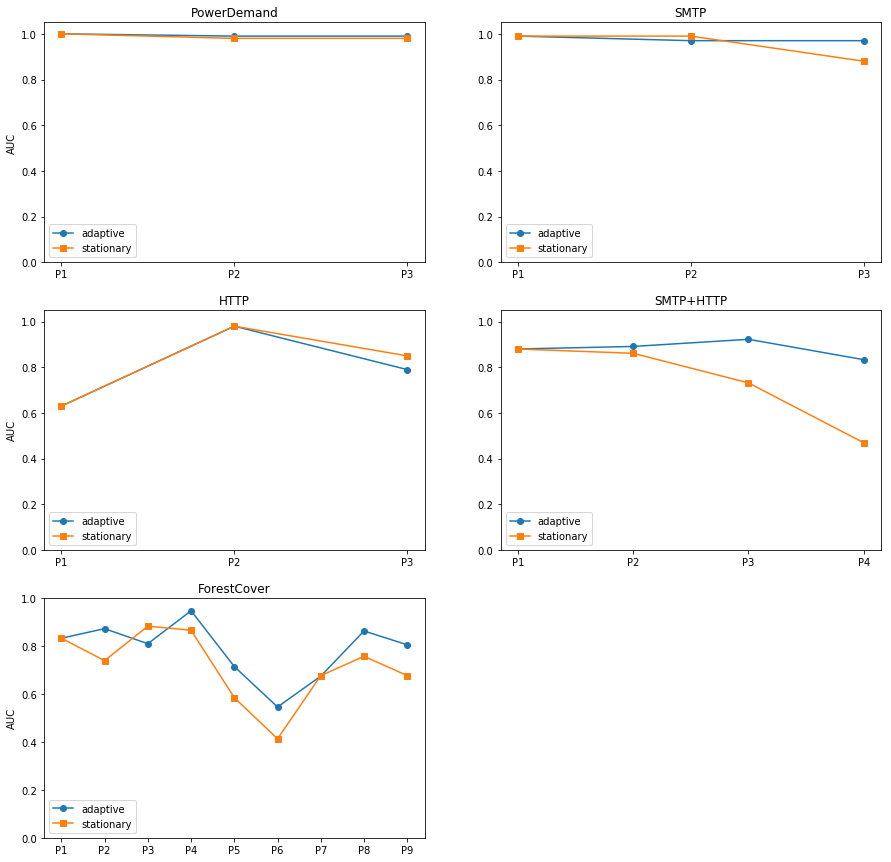
\includegraphics[width=15cm, height=15cm]{auc_retrain}
\caption[AUC comparation between stationary and adaptive models over stream]{AUC comparation between stationary and adaptive models over stream. The x-axis represents specific periods over stream. For example, P1 is the period from beginning to the first retraining, and P2 is the the period between first and second retraining etc.}
\label{fig:auc_retrain}
\end{figure}

\Fref{fig:runtime} shows the run time used for both stationary models and adaptive models for each data set. The updating takes more time for HTTP, SMTP+HTTP and ForesrCover than PowerDemand and SMTP is due to that larger datasets take more time for prediction, and trigger more updating events. And for each retraining, the retrain buffers also contain larger retraining sets.



\begin{figure}[h]
\centering
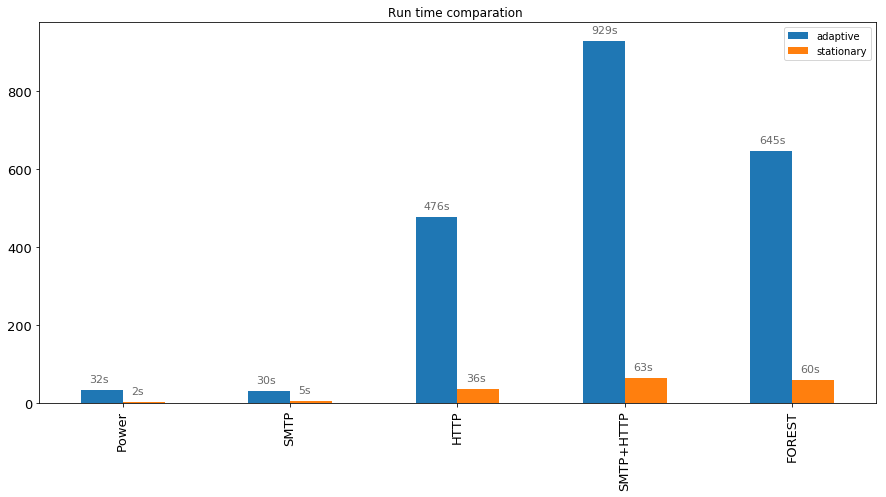
\includegraphics[width=15cm, height=7cm]{runtime}
\caption[Run time statistics]{Run time statistics}
\label{fig:runtime}
\end{figure}


\section{Synthetic example}
\label{sec:synthetic}

In order to show the benefit of model updating over the stream, we demonstrate the online learning process of the small set PowerDemand in this section. The PowerDemand dataset does not contain clear incremental or sudden concept drift, but the normal patterns still different slightly to each other. The lack of overall impression during the model initialization phase can lead to failures during the online phase. 

\subsection{Anomaly detection over stream}
\label{sec:detection}

Generally, the autoencoder reconstructs normal data with relative lower reconstruction error while anomaly data with significant larger reconstruction error. \Fref{fig:power_re} demonstrates two typical data windows (weeks) in PowerDemand, one normal and one anomaly. The Monday of anomaly week (right) is a special data, which has an abnormally low power demand. Even so, the autoencoder still reconstructs the Monday as usual with a higher score, therefore the reconstruction error is obviously larger on Monday, and the model labels this week as anomaly.\\

\begin{figure}[h]
\centering
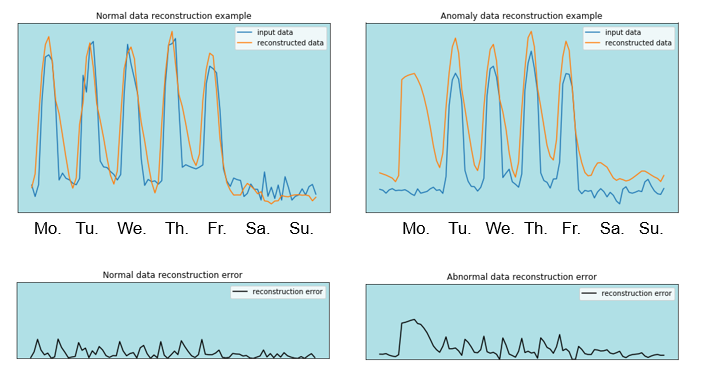
\includegraphics[width=12cm, height=8cm]{power_na}
\caption[Reconstruction error of PowerDemand data]{Reconstruction error of PowerDemand data}
\label{fig:power_re}
\end{figure}

Even there will be concept drift over the stream, which will lead to an entirely increase or decrease in the input side, and the decoder output side remaining, our model can still deal with this problem with its online parameter updating ability. While the anomaly scores are calculated by the mahalanobis distance to the estimated normal distribution of normal data reconstruction errors in the validation set, by every model updating, the model estimates new normal distribution and relevant parameters with the latest collected validation set, so that the reconstruction error based anomaly detection is robust against concept drift.\\



\subsection{Reaction of concept drift}
\label{sec:reaction}

\Fref{fig:power_retraining} shows 3 continual days power demand in normal state. Due to the lack of knowledge for current pattern, the autoencoder reconstructs the input time series higher than desired on day 1 (left diagram). This could be caused by seasonal changes on the power demand, which is slightly, gradually, and would potentially cause misclassification. The increase of normal data reconstruction error makes the margin between two classification classes smaller, and harder to make decision. As a consequence, the model retraining process is triggered after the second day with last seen data in the buffers, and the model performs well again on the third day.

\begin{figure}[h]
\centering
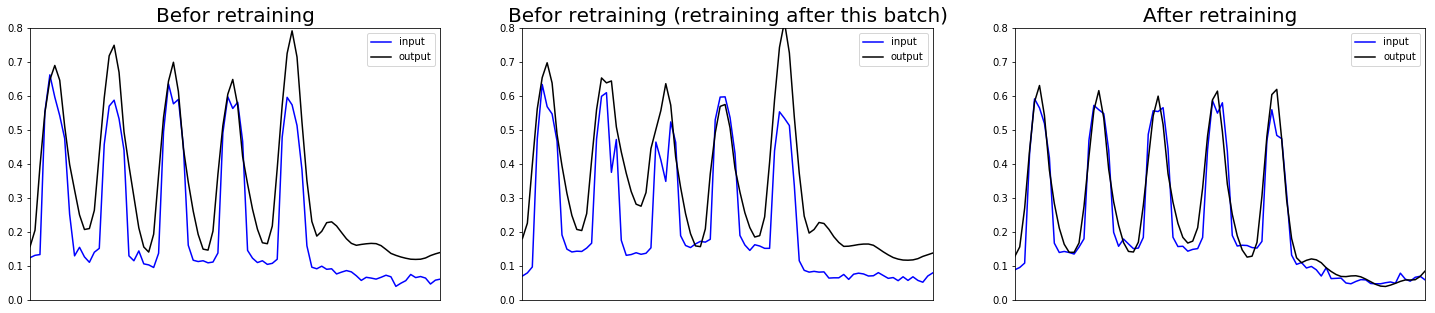
\includegraphics[width=15cm, height=4cm]{power_retraining}
\caption[Retraining effect on PowerDemand dataset]{Retraining effect on PowerDemand dataset}
\label{fig:power_retraining}
\end{figure}

\subsection{Model updating}
\label{sec:retrainig}

During the online phase, the model is retrained two times, before batch No.10 and No. 27. After retraining, the normal data reconstruction error becomes lower while for abnormal data becomes higher, so that the classification becomes easier.

\begin{figure}[h]
\centering
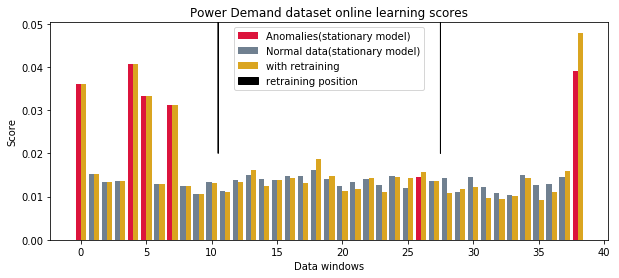
\includegraphics[width=10cm, height=4cm]{power_online_score}
\caption[PowerDemand dataset online learning scores]{PowerDemand dataset online learning scores. For each window, the anomaly score is the highest pointwise scores within the window}
\label{fig:power_online}
\end{figure}

After each updating process, the parameters mu, sigma and threshold of anomaly scores are also updated. \Fref{fig:parachanges} shows the parameter changes over the stream. As there is no clear concept drift during the power demand stream, the parameters change just slightly in oder to learn latest knowledge from the retrain buffer. 

\begin{figure}[h]
\centering
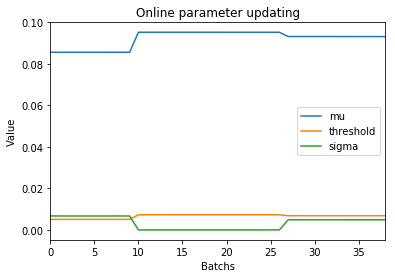
\includegraphics[width=6cm, height=4cm]{para_update}
\caption[PowerDemand dataset online parameter updating]{PowerDemand dataset online parameter updating}
\label{fig:parachanges}
\end{figure}



\section{Model retraining}
\label{sec:retraining}

\subsection{Reaction of sudden and drastic concept drift}
\label{sec:reaction}

The main advantage of online model is its ability to take reaction against sudden data distributional changes over time. The SMTP+HTTP data set is composed by directly connecting HTTP set after SMTP, so there is a sudden concept drift in between. The model is initialized with only SMTP data, so HTTP is completely unknown knowledge for the model. \Fref{fig:smtp+http} shows the scores for both normal and abnormal data over the SMTP+HTTP stream. In the beginning, only SMTP data in the stream, and partially used for model initialization. In the online prediction phase, once the HTTP data arrives, the first peak of normal data scores’ curve appears, and then the model updating is triggered, with buffer data being few hard SMTP data and most HTTP data. After the first model updating, the performance of model is still suboptimal due to the lack of enough HTTP data, therefore there are two further model updating process triggered during the following stream. As a result, the overall anomaly detection for SMTP+HTTP stream is good only except the short period after concept drift. The model updating are triggered in time after concept drift, and afterwards no redundant updating are triggered.

\begin{figure}[h]
\centering
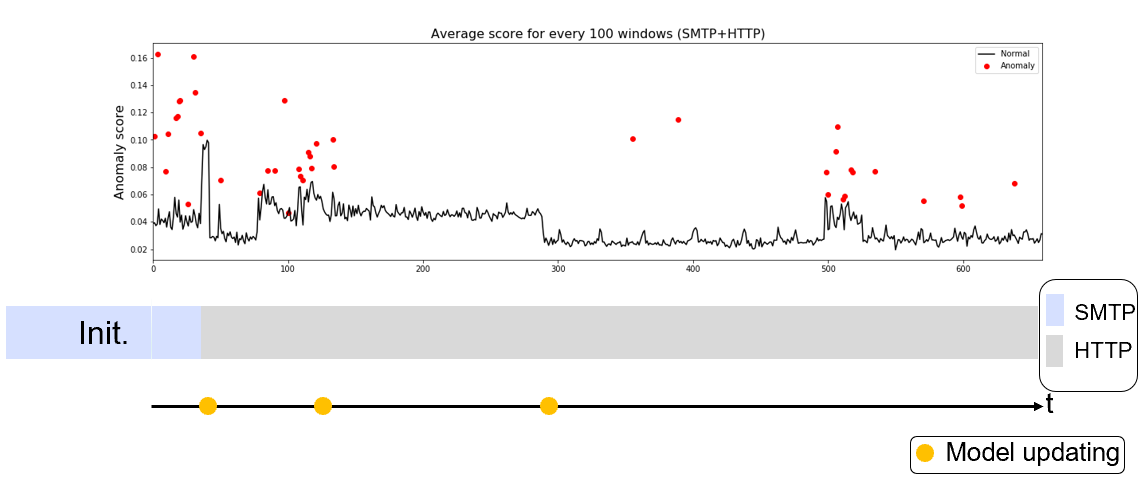
\includegraphics[width=15cm, height=7cm]{sh_conceptdrift}
\caption[SMTP+HTTP stream concept drift]{SMTP+HTTP stream concept drift.}
\label{fig:smtp+http}
\end{figure}

\subsection{Reaction of serial concept drift}
\label{sec:reaction}

Sometimes concept drift over the stream are slight, periodically, and potentially repeated. A single slight concept drift may not be able to trigger the retraining, but new knowledge should be saved into retraining buffer, so that once the model retrained with the fresh knowledge, tshe model should perform well when the same concept drift happens. We experiment with the ForestCover dataset. There are 7 kinds of forest cover types as labels. We take the least TYPE4 as anomaly while the rest 6 kinds as normal. The ForestCover stream is generated type by type, as shown in the bottom chart of \Fref{fig:fcd}. During the beginning phase, TYPE1 data appears in the stream, part of which is used for model initialization. Afterwards follows instances from TYPE2, TYPE3, TYPE5, TYPE6, TYPE7 and finally TYPE2 appears again during the ending phase. Anomaly data (TYPE4) is randomly distributed in the stream. Because the model is only initialized with TYPE1 data, every appearance of a new cover type will potentially cause a performance decrease. The concept drift under this setting is then the type changes over stream. \\

\begin{figure}[h]
\centering
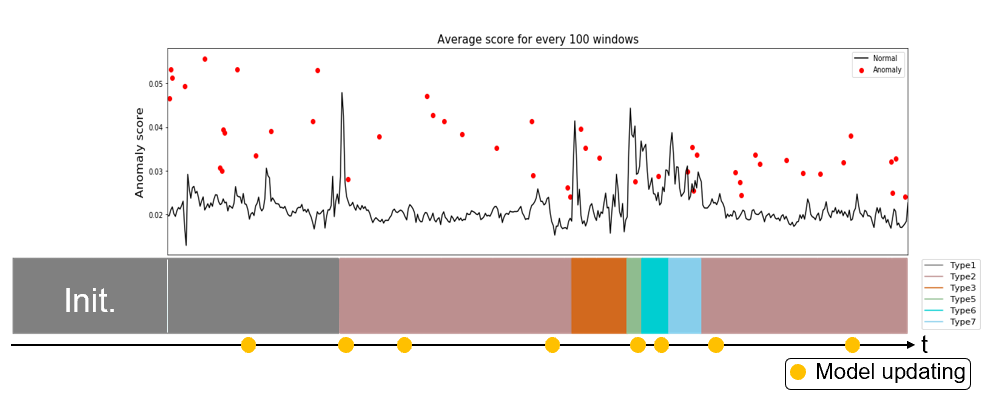
\includegraphics[width=15cm, height=8cm]{forestconceptdrift}
\caption[ForestCover stream concept drift]{ ForestCover stream concept drift. The chart on the bottom shows the cover type over the stream. The top chart shows average anomaly scores for every 100 windows}
\label{fig:fcd}
\end{figure}

The points on the time axis in \Fref{fig:fcd} indicates the model updating. In the anomaly score chart, the scores for anomaly data are generally larger than normal data except when concept drifts take place. Once data stream from a new cover type appears in the stream, there are always peaks in the normal data score plot, and the difference to anomaly data scores decreases. After performance being impacted, the normal buffer is filled with hard windows shortly, that triggers the model updating quickly after the concept drift. \\

During the experiment, there are two cases delay the updating. Firstly, because of the fixed size of buffer, if a model updating is just triggered shortly before a concept drift, then the hard windows from new cover type need more time to fill the buffer and trigger updating. In \Fref{fig:fcd}, before TYPE3 arrive, there was a updating at the end of TYPE2, and buffered was emptied, so that the model didn’t take any action against the concept drift. Secondly, if a concept drift only appears in a short period, e.g. the TYPE7, which is also not enough to fill the buffer and trigger updating. However, under both aforementioned cases, the new information of concept drift, namely the new cover types, are stored in the buffer, and will be used for next model updating. If the concept drift missed model updating due to too short appearance period, we suppose that this would also not cause catastrophic effect over the stream prediction.\\


\subsection{Summary}
\label{sec:summary}

In this section, we experimented out online LSTMs-Autoencoder model with five different streaming data. With the PowerDemand dataset, we demonstrated a synthetic example of our model, which shows the reconstruction error based anomaly detection mechanism and how the reconstruction adapt to new coming streaming data through model updating. Furthermore, we use the two dataset that contains obvious concept drift, SMTP+HTTP and ForestCover. The model reacts quickly to sudden and drastic concept drift, and potentially more updating will be triggered after concept drift to catch enough valuable information from the drifted stream. And when multiple concept drifts happen temporally and shortly, the model misses some of them, but the fresh information of those concept drifts are still accumulated to the buffer and used by next updating.








\chapter{Conclusion}
\label{chap:conclusion}




%APPENIX
\appendix

%REFERENCE
\bibliographystyle{plain}
\bibliography{referenzen}

\end{document}
